% ============================================================
%  Chapter 2 ---'' The Type Zoo: A Catalog of Types
%  "Type Theory from the Ground Up"
% ============================================================
\chapter{The Type Zoo --- A Catalog of Types}
\label{ch:type-zoo}

In Chapter~1 we asked the fundamental question: \emph{what is a type?} We saw two
complementary answers --- types as sets of values, and types as behavioral
contracts --- and we talked about what it means for a type system to be sound.
That was the philosophical warm-up.

Now we roll up our sleeves. This chapter is a guided tour of the \emph{type zoo}:
every major species of type you will encounter in modern programming languages and
in type theory itself. Some of these animals will be familiar, some surprising, and
a few might seem a little exotic at first. By the end of the chapter you will have a
systematic vocabulary for talking about types, and --- crucially --- you will
understand \emph{why} each species exists and what problem it solves.

We will keep one eye on C++ throughout, because C++ is unusually rich in its
type-system features (for better and worse), and keeping a concrete language in
mind makes the abstract ideas stick. Where C++ falls short or does something
surprising, we will say so plainly.

Ready? Step through the gate.

% ============================================================
\section{Before We Start: Cardinality}
\label{sec:cardinality-intro}
% ============================================================

There is one concept that will appear again and again as we walk through the zoo,
so let us define it cleanly right at the start.

\begin{definition}
The \textbf{cardinality} of a type \(T\), written \(|T|\), is the number of
distinct values that inhabit \(T\). In set-theoretic terms it is simply the size
of the corresponding set.
\end{definition}

Cardinality is a surprisingly powerful lens. Once you know the cardinality of a
type, you immediately know things like:
\begin{itemize}
  \item how many bits you \emph{need} to represent a value of that type;
  \item how many distinct functions exist between two types;
  \item whether two types are ``morally the same'' (isomorphic) even if they look
        different on the surface.
\end{itemize}

You do not need any advanced mathematics to use cardinality --- just the ability
to count. Let us start counting.

% ============================================================
\section{Primitive Types --- The Atoms of the Type Zoo}
\label{sec:primitive-types}
% ============================================================

Every type system is built on a foundation of \emph{primitive} (or \emph{base})
types: types that the language defines directly, without assembling them from
smaller pieces. They are the atoms from which everything else is constructed.

\subsection{Integers}

The most common primitive type is some form of integer. In mathematics, the
integers \(\mathbb{Z}\) are infinite, but in a computer everything lives in a
finite amount of memory, so every practical integer type has a fixed width.

\begin{cppconnection}[Integer types in C++]
C++ offers a bewildering variety of integer types:
\begin{lstlisting}[style=cpp]
bool        b = true;      // 1 bit of information (see Section 2.4)
char        c = 'A';       // typically 8 bits, character encoding
short       s = 32767;     // at least 16 bits
int         i = 42;        // at least 16 bits, usually 32
long        l = 1000000L;  // at least 32 bits
long long   ll = 9e18;     // at least 64 bits

// Explicit-width types from <cstdint> ---'' prefer these
int8_t   i8  = -128;
uint8_t  u8  = 255;
int16_t  i16 = -32768;
uint16_t u16 = 65535;
int32_t  i32 = 2147483647;
uint64_t u64 = 18446744073709551615ULL;
\end{lstlisting}
\end{cppconnection}

Let us count. A type represented by \(n\) bits can hold \(2^n\) distinct bit
patterns, giving it cardinality \(2^n\).

\begin{center}
\begin{tabular}{lcc}
\hline
\textbf{Type} & \textbf{Width} & \textbf{Cardinality} \\
\hline
\code{uint8\_t}  & 8 bits  & \(2^8 = 256\) \\
\code{int8\_t}   & 8 bits  & \(2^8 = 256\) \\
\code{uint16\_t} & 16 bits & \(2^{16} = 65{,}536\) \\
\code{int32\_t}  & 32 bits & \(2^{32} \approx 4.3 \times 10^9\) \\
\code{int64\_t}  & 64 bits & \(2^{64} \approx 1.8 \times 10^{19}\) \\
\hline
\end{tabular}
\end{center}

Notice that \code{uint8\_t} and \code{int8\_t} have the \emph{same} cardinality:
256. The difference is not in \emph{how many} values they hold, but in \emph{which}
values they hold. \code{uint8\_t} covers \(0\) to \(255\); \code{int8\_t} covers
\(-128\) to \(127\). Two different sets, same size --- a type-theory isomorphism.

\begin{keyinsight}[Signed vs.\ unsigned: same cardinality{,} different values]
Signed and unsigned variants of the same bit-width are isomorphic as types ---
there is a one-to-one correspondence between their values. The type system
distinguishes them because they have different \emph{behaviors} (arithmetic
wrapping, comparison, etc.), not because one is ``bigger'' than the other.
\end{keyinsight}

\subsection{Floating-Point Types}

Floating-point types represent approximations to real numbers. C++ has
\code{float} (32-bit, IEEE 754 single precision), \code{double} (64-bit, double
precision), and \code{long double} (80- or 128-bit, implementation-defined).

From a cardinality standpoint, \code{float} has \(2^{32} = 4{,}294{,}967{,}296\)
bit patterns, just like \code{uint32\_t}. But floating-point encodes something
qualitatively different: numbers spread across a huge range (roughly
\(\pm 3.4 \times 10^{38}\) for \code{float}), with higher density near zero.
Special values like \code{NaN} (Not a Number) and \code{Infinity} are members
of the type --- which can be surprising.

\begin{warning}[Floating-point is not math]
\code{float} is \emph{not} a subset of the real numbers. It is a specific finite
set of representable values with carefully defined arithmetic rules. Two values
that look equal in mathematics may differ as floats:
\begin{lstlisting}[style=cpp]
double a = 0.1 + 0.2;
double b = 0.3;
// a == b is FALSE on most hardware
\end{lstlisting}
Type theory cares about this because it means the \emph{specification} of
\code{double} (the set of values and operations) differs from what mathematicians
mean by ``real number.'' This distinction matters when you reason about programs.
\end{warning}

\subsection{Characters}

A \code{char} represents a single character. In C++ it is typically 8 bits, giving
cardinality 256. But character types are really just integers wearing a costume:
the type system gives them a distinct name to signal \emph{intent} (``this
represents a character''), but the underlying representation is numeric.

Modern C++ adds \code{char8\_t}, \code{char16\_t}, and \code{char32\_t} for
Unicode encodings, each with the corresponding cardinality \(2^8\), \(2^{16}\),
\(2^{32}\).

\begin{intuition}
Primitive types are small, fast, and directly supported by the hardware. Their
cardinalities are always powers of two because computer memory is organized in
bits. All the more complex types we meet in this chapter are ultimately built
by combining and constraining these primitives.
\end{intuition}

% ============================================================
\section{The Unit Type --- Exactly One Value}
\label{sec:unit-type}
% ============================================================

Here is a type you have almost certainly used without knowing its formal name.

\begin{definition}
The \textbf{unit type}, written \(\Unit\) in type theory (or \code{()} in Haskell
and Rust), is the type with exactly one value. That single value is often also
called ``unit'' and written \code{()}.
\[
  |\Unit| = 1
\]
\end{definition}

Why would anyone want a type with only one value? Let us think carefully.

A value carries \emph{information}. If a type has \(n\) possible values, then
knowing which value you have gives you \(\log_2 n\) bits of information. A type
with one value carries \(\log_2 1 = 0\) bits of information. A value of type
\(\Unit\) tells you \emph{nothing} --- because it could only ever be the one
thing it is.

\begin{keyinsight}[Unit carries no information]
A function that returns \(\Unit\) is interesting only for its \emph{side effects}.
Since the return value is always the single element \code{()}, it conveys zero
information to the caller. This makes \(\Unit\) the perfect return type for
``do something and report nothing'' operations: printing, writing to a file,
updating a counter.
\end{keyinsight}

\subsection{Unit in C++: The \code{void} Situation}

C++ does not have a clean unit type, but \code{void} plays a similar role ---
with some important caveats.

\begin{lstlisting}[style=cpp]
void print_greeting() {
    std::cout << "Hello, type theorist!\n";
    // No return value
}
\end{lstlisting}

In type theory, a function \(f : A \to \Unit\) is a perfectly ordinary function
with a well-typed return value --- it just happens that the return value carries
no information. In C++, \code{void} is handled specially by the compiler: you
cannot declare a variable of type \code{void}, you cannot pass a \code{void}
value to a function, and you cannot do much of anything with it.

This asymmetry causes real pain in generic (template) code:

\begin{lstlisting}[style=cpp]
// This does NOT compile in C++ if f() returns void:
template <typename F>
auto call_and_log(F f) {
    auto result = f();   // ERROR if f returns void
    std::cout << "Called f\n";
    return result;
}
\end{lstlisting}

Languages with a proper \(\Unit\) type (Haskell, Rust, OCaml) do not have this
problem, because \code{()} is a genuine first-class value. C++23 partially
addresses this with \code{std::expected<void, E>} and similar constructs, but
the fundamental asymmetry remains.

\begin{cppconnection}[Simulating Unit in C++]
If you ever need a proper unit type in C++ (for example, in a generic data
structure), you can define one:
\begin{lstlisting}[style=cpp]
struct Unit {
    // No members ---'' exactly one value exists: Unit{}
    bool operator==(const Unit&) const { return true; }
};

// Now Unit{} is a genuine first-class value
Unit u = Unit{};
std::vector<Unit> v(10); // Ten "unit" values
\end{lstlisting}
This pattern shows up in practice in template metaprogramming.
\end{cppconnection}

\subsection{An Analogy: The Light Switch With One Position}

Imagine a light switch that is \emph{welded in place}. It cannot be flipped.
You can look at it, touch it, pass it around --- but you always get the same
answer: ``stuck.'' That switch is the unit type. Its existence is meaningful
(you know \emph{something} exists), but its state carries no news.

% ============================================================
\section{The Bottom Type --- Exactly Zero Values}
\label{sec:bottom-type}
% ============================================================

If the unit type has one value and feels minimalist, get ready for the bottom
type, which takes minimalism to its logical extreme.

\begin{definition}
The \textbf{bottom type}, written \(\bot\) (pronounced ``bottom'') in type theory,
is the type with \emph{zero} values. No value inhabits \(\bot\).
\[
  |\bot| = 0
\]
\end{definition}

This sounds absurd. How can you have a type with no values? What would a variable
of type \(\bot\) even contain?

The answer is: nothing. A variable of type \(\bot\) can never be given a value,
which means \emph{it can never exist at runtime}. But this is precisely what
makes \(\bot\) useful: it is the type of computations that never \emph{finish}.

\subsection{The Principle of Explosion}

Here is a beautiful logical fact. In classical logic, from a false premise you
can derive anything. The type-theoretic analogue is:

\begin{keyinsight}[The principle of explosion]
If you somehow have a value of type \(\bot\), you can produce a value of
\emph{any} type. This is written:
\[
  \text{absurd} : \bot \to A \quad \text{for any type } A
\]
The function \text{absurd} is not a contradiction --- it is vacuously valid,
because its premise (a \(\bot\) value) can never actually occur. You will never
be called upon to produce the \(A\), because you will never receive the \(\bot\).
\end{keyinsight}

This shows that \(\bot\) is the \emph{subtype of every type}: it is at the very
bottom of the type hierarchy (hence the name). Every type has at least as many
values as \(\bot\) (which has zero), so \(\bot \subseteq A\) for every \(A\).

\subsection{Bottom in C++: Functions That Never Return}

C++ does not have a named bottom type, but it has a way to mark functions that
behave like one.

\begin{lstlisting}[style=cpp]
#include <cstdlib>
#include <stdexcept>

[[noreturn]] void fatal_error(const std::string& msg) {
    std::cerr << "Fatal: " << msg << "\n";
    std::abort();   // Program terminates ---'' never returns
}

[[noreturn]] void throw_always() {
    throw std::runtime_error("This always throws");
}
\end{lstlisting}

The \code{[[noreturn]]} attribute tells the compiler: ``this function's return
type is, conceptually, \(\bot\).'' The compiler uses this information to suppress
spurious warnings about missing \code{return} statements and to generate better
code around call sites.

\begin{lstlisting}[style=cpp]
int divide(int a, int b) {
    if (b == 0) fatal_error("division by zero");
    return a / b;  // Compiler knows we reach here only if b != 0
}
\end{lstlisting}

In languages like Rust and Haskell the bottom type is explicit. Rust spells it
\code{!} (the ``never'' type):

\begin{lstlisting}[style=haskell]
-- Haskell: undefined has type a for any a ---'' it is bottom
-- because it diverges (throws an error) when evaluated
bottom :: a
bottom = error "I never produce a value"
\end{lstlisting}

\begin{warning}[Divergence and \(\bot\)]
In a language with non-termination (like most real languages), every type is
secretly ``infected'' with \(\bot\): any expression might loop forever or throw
an exception. Denotational semantics deals with this by explicitly adding
\(\bot\) to every type's domain. For our purposes, you can think of \(\bot\)
as the type of ``clearly intentional non-termination'' --- panics, aborts,
infinite loops that are deliberate by design.
\end{warning}

% ============================================================
\section{The Boolean Type --- Two Values, Infinite Consequences}
\label{sec:boolean-type}
% ============================================================

After the extremes of zero and one, we meet the first type that is genuinely
\emph{interesting}: the Boolean.

\begin{definition}
The \textbf{Boolean type} \(\Bool\) has exactly two values: \(\textit{true}\)
and \(\textit{false}\).
\[
  |\Bool| = 2
\]
\end{definition}

Booleans are the bedrock of logic and control flow. Every \code{if} statement,
every \code{while} loop, every short-circuit \code{\&\&} and \code{||} operates
on Booleans (or things implicitly convertible to them).

\begin{lstlisting}[style=cpp]
bool is_prime(int n) { /* ... */ }
bool is_even(int n)  { return n % 2 == 0; }

bool result = is_prime(7) && is_even(4); // false && true = false
\end{lstlisting}

\subsection{Booleans and Logic}

The connection between Booleans and classical propositional logic is tight.
Each Boolean operation corresponds to a logical connective:

\begin{center}
\begin{tabular}{lll}
\hline
\textbf{Operation} & \textbf{C++ syntax} & \textbf{Logic} \\
\hline
AND & \code{a \&\& b} & \(a \land b\) \\
OR  & \code{a || b}  & \(a \lor b\) \\
NOT & \code{!a}       & \(\lnot a\) \\
XOR & \code{a \^{} b} & \(a \oplus b\) \\
Implication & \code{!a || b} & \(a \Rightarrow b\) \\
\hline
\end{tabular}
\end{center}

This correspondence is not a coincidence. It is a deep structural relationship
called the \emph{Curry--Howard correspondence}, which we will explore in depth
in Chapter~8. For now, file away the intuition: \emph{types are propositions,
and values are proofs}.

\begin{keyinsight}[Two values is the minimum for interesting computation]
\(\Unit\) (one value) is too small to branch on: all paths lead to the same
place. \(\Bool\) (two values) is the minimum size needed for a type to support
a non-trivial \code{if}. This is why \(\Bool\) is sometimes called the
``universal bit'' --- it is the irreducible quantum of decision.
\end{keyinsight}

\subsection{Counting Functions on Booleans}

How many distinct functions are there from \(\Bool\) to \(\Bool\)? A function
must specify an output for each possible input. \(\Bool\) has 2 inputs, and each
output can be one of 2 values, so there are \(2^2 = 4\) such functions:

\begin{center}
\begin{tabular}{llll}
\hline
\textbf{Name} & \(\textit{false} \mapsto\) & \(\textit{true} \mapsto\) & \textbf{C++ expression} \\
\hline
Constant false & false & false & \code{[](bool) \{ return false; \}} \\
Identity       & false & true  & \code{[](bool b) \{ return b; \}} \\
Negation       & true  & false & \code{[](bool b) \{ return !b; \}} \\
Constant true  & true  & true  & \code{[](bool) \{ return true; \}} \\
\hline
\end{tabular}
\end{center}

This ``\(|B|^{|A|}\)'' counting formula will reappear when we talk about
function types in Section~\ref{sec:function-types}.

% ============================================================
\section{Enumeration Types --- Named Finite Sets}
\label{sec:enum-types}
% ============================================================

Now we take one step up in sophistication. An enumeration type (``enum'') is a
type whose values are a specific, named, finite set that you define.

\begin{definition}
An \textbf{enumeration type} with \(n\) enumerators is a type with cardinality
\(n\). Its values are distinguished by name rather than by numeric meaning.
\end{definition}

\begin{lstlisting}[style=cpp]
// C-style enum ---'' use with caution (see below)
enum Color { Red, Green, Blue };        // |Color| = 3

// Strongly-typed enum class ---'' strongly preferred
enum class Direction { North, South, East, West };  // |Direction| = 4
enum class Weekday   { Mon, Tue, Wed, Thu, Fri, Sat, Sun }; // |Weekday| = 7
\end{lstlisting}

The cardinality of an enum is simply the number of enumerators you list. Nothing
complicated here --- but the consequences for correctness are significant.

\subsection{Why Enums Matter for Type Safety}

Consider a function that takes a direction:

\begin{lstlisting}[style=cpp]
// Version 1: using int ---'' anything can be passed
void move(int direction) { /* ... */ }
move(0);    // OK? Which direction is 0?
move(99);   // Compiles fine. Disaster at runtime.

// Version 2: using enum class ---'' the type IS the documentation
void move(Direction d) { /* ... */ }
move(Direction::North);  // Correct and clear
move(99);                // COMPILE ERROR ---'' 99 is not a Direction
\end{lstlisting}

The \code{enum class} version encodes the set of valid values directly in the
type. The compiler enforces that only those values can be passed. This is
\emph{type-driven design}: letting the type system catch mistakes.

\begin{cppconnection}[Old-style \code{enum} vs \code{enum class}]
Old C-style enums have two problems:
\begin{enumerate}
  \item Their enumerators leak into the surrounding scope (\code{Red}, not
        \code{Color::Red}), causing name collisions.
  \item They implicitly convert to \code{int}, undermining type safety.
\end{enumerate}
\code{enum class} (introduced in C++11) fixes both. Always prefer \code{enum class}
in new code.
\end{cppconnection}

\begin{keyinsight}[Enums are finite types with named inhabitants]
An \code{enum class} is simply a type whose value set you enumerate by name.
It is not a number; it just happens to be stored as one internally. The type
system's job is to ensure you never treat it as an arbitrary number.
\end{keyinsight}

\subsection{The Underlying Type}

In C++, every \code{enum} has an \emph{underlying type} (by default, some
\code{int} variant) that determines its representation. You can specify it:

\begin{lstlisting}[style=cpp]
enum class Status : uint8_t {
    Ok      = 0,
    Warning = 1,
    Error   = 2
};
// sizeof(Status) == 1 byte
// |Status| == 3 (only Ok, Warning, Error are valid ---'' not all 256 bit patterns!)
\end{lstlisting}

This highlights a key point: the cardinality of \code{Status} is 3, not 256,
even though the underlying storage has 256 possible bit patterns. The type system
is telling you which of those 256 patterns are \emph{meaningful}. The rest are
invalid --- and accessing them is undefined behavior.

% ============================================================
\section{Product Types --- Combining with AND}
\label{sec:product-types}
% ============================================================

We have met individual types. Now we start combining them. The first and most
natural way to combine types is to ask: what if I need \emph{both} an \(A\)
\emph{and} a \(B\)?

\begin{definition}
The \textbf{product type} of \(A\) and \(B\), written \(A \times B\), is the
type whose values are ordered pairs \((a, b)\) where \(a : A\) and \(b : B\).
\[
  |A \times B| = |A| \times |B|
\]
\end{definition}

The name ``product'' is not an accident: the cardinality of the combined type is
the \emph{product} of the individual cardinalities. If \(A\) has 3 values and
\(B\) has 4 values, then \(A \times B\) has 12 values --- one for each
combination.

\subsection{Structs and Classes as Product Types}

In C++, \code{struct} and \code{class} are the primary mechanism for product
types.

\begin{lstlisting}[style=cpp]
struct Point {
    double x;   // type: double
    double y;   // type: double
};
// |Point| = |double| * |double| = 2^64

struct Person {
    std::string name;
    uint32_t    age;
    bool        is_student;
};
// |Person| = |string| * |uint32_t| * |bool|
//          = huge    * 2^32       * 2
\end{lstlisting}

A \code{Person} value contains a \code{name} \emph{and} an \code{age} \emph{and}
an \code{is\_student}. All three fields are present simultaneously. That is the
essence of a product type.

\begin{keyinsight}[Struct = AND type]
When you write \code{struct \{ A a; B b; \}}, you are creating a type that means
``has an A \emph{and} a B.'' The total number of possible states is $|A| \times |B|$
because each field is independent and can take any of its values.
\end{keyinsight}

\subsection{Tuples}

A \emph{tuple} is an anonymous product type --- a product type without field
names, where fields are accessed by position.

\begin{lstlisting}[style=cpp]
#include <tuple>
#include <utility>  // for std::pair

std::pair<int, bool> p = {42, true};
auto x = p.first;   // 42
auto y = p.second;  // true

std::tuple<int, bool, double> t = {1, false, 3.14};
auto a = std::get<0>(t);  // 1
auto b = std::get<1>(t);  // false
auto c = std::get<2>(t);  // 3.14
\end{lstlisting}

\begin{example}
Consider the type \(\Bool \times \Bool\). Its cardinality is \(2 \times 2 = 4\).
The four inhabitants are:
\[
  (\textit{false}, \textit{false}), \quad
  (\textit{false}, \textit{true}),  \quad
  (\textit{true},  \textit{false}), \quad
  (\textit{true},  \textit{true})
\]
This is the same as the truth table for a binary Boolean connective --- no
coincidence.
\end{example}

\subsection{Projection Functions}

Every product type \(A \times B\) comes with two canonical functions for
extracting components, called \emph{projections}:
\[
  \pi_1 : A \times B \to A \qquad \pi_2 : A \times B \to B
\]
In C++ these are \code{.first}/\code{.second} for pairs, or \code{std::get<N>}
for tuples.

\subsection{Nested Products and Flat Products}

Products can be nested:
\[
  (A \times B) \times C \quad \text{vs.} \quad A \times (B \times C) \quad
  \text{vs.} \quad A \times B \times C
\]
These three are \emph{not} identical types, but they are isomorphic --- you can
convert between them without loss of information. This is the type-theoretic
analogue of the associativity of multiplication.

A struct with many fields is really just a deeply nested or flat product type.
The order of fields does not change the cardinality, but it does change the
type's identity (two structs with the same fields in different orders are
distinct types in C++).

% ============================================================
\section{Sum Types --- Combining with OR}
\label{sec:sum-types}
% ============================================================

Product types capture ``and.'' The dual notion captures ``or.''

\begin{definition}
The \textbf{sum type} (also called \textbf{tagged union} or \textbf{coproduct})
of \(A\) and \(B\), written \(A + B\), is the type whose values are
\emph{either} a value from \(A\) \emph{or} a value from \(B\) --- but never
both simultaneously --- along with a tag indicating which.
\[
  |A + B| = |A| + |B|
\]
\end{definition}

Again the name matches the arithmetic: the cardinality of a sum type is the
\emph{sum} of the individual cardinalities.

\subsection{Tagged vs.\ Untagged Unions}

There are two flavors of union type, and they are very different in safety.

\paragraph{Untagged union (C++ \code{union}).}
A C++ \code{union} stores one of several types in the same memory, but does
\emph{not} record which type is currently stored.

\begin{lstlisting}[style=cpp]
union Dangerous {
    int    i;
    float  f;
    double d;
};

Dangerous u;
u.i = 42;
double x = u.d;  // UNDEFINED BEHAVIOR: we wrote int, read double
\end{lstlisting}

This is wildly unsafe. The programmer must externally track which member is
active. If they get it wrong, the result is undefined behavior. Untagged
unions have cardinality \(\max(|A|, |B|)\) in terms of storage, but the type
system provides \emph{no} safety --- any value can be read as any member.

\paragraph{Tagged union (\code{std::variant}).}
\code{std::variant} is a safe, tagged union introduced in C++17. It stores
both the value \emph{and} an internal tag indicating which alternative is active.

\begin{lstlisting}[style=cpp]
#include <variant>
#include <string>

std::variant<int, float, std::string> v;

v = 42;                       // v holds an int
int i = std::get<int>(v);     // OK

v = "hello";                  // v now holds a string
// int j = std::get<int>(v);  // THROWS std::bad_variant_access

// Safe access with std::visit
std::visit([](auto&& val) {
    using T = std::decay_t<decltype(val)>;
    if constexpr (std::is_same_v<T, int>)
        std::cout << "int: " << val << "\n";
    else if constexpr (std::is_same_v<T, std::string>)
        std::cout << "string: " << val << "\n";
}, v);
\end{lstlisting}

\begin{keyinsight}[Sum type = OR type]
\code{std::variant<A, B>} means ``this value is \emph{either} an A \emph{or}
a B, and I can always tell which.'' The tag is the crucial ingredient: it is
what makes the type safe. Without the tag (raw \code{union}), you have a
type with no safety guarantees.
\end{keyinsight}

\subsection{Optional as a Special Sum Type}

A tremendously important sum type is \(\mathtt{Optional}(A)\), which means
``either a value of type \(A\), or nothing at all.''

\[
  \mathtt{Optional}(A) = A + \Unit
\]

In C++ this is \code{std::optional<A>}:

\begin{lstlisting}[style=cpp]
#include <optional>

std::optional<int> find_user_id(const std::string& name) {
    if (name == "Alice") return 42;
    return std::nullopt;   // The "nothing" case
}

auto id = find_user_id("Bob");
if (id) {
    std::cout << "Found: " << *id << "\n";
} else {
    std::cout << "Not found\n";
}
\end{lstlisting}

\[
  |\mathtt{optional}\langle A \rangle| = |A| + 1
\]

The \(+1\) is the \code{nullopt} value. \code{std::optional<bool>} has cardinality
3: \code{false}, \code{true}, and \code{nullopt}.

\begin{warning}[Null pointers are a broken optional]
C's null pointer (\code{nullptr}) was intended to serve the role of \code{nullopt}:
to signal ``no valid value.'' But a raw pointer type \code{T*} does not make
this explicit in the type system. Every raw pointer is \emph{silently} optional,
even when you did not intend it. Null pointer dereferences are the result.
\code{std::optional<T>} makes the optionality \emph{explicit}: if you have a
non-optional value, no null check is needed --- the type guarantees it.
\end{warning}

\subsection{Result/Either Types}

Another common sum type is a \emph{result type}: either success or failure.

\begin{lstlisting}[style=cpp]
#include <expected>  // C++23

std::expected<int, std::string> parse_int(const std::string& s) {
    try {
        return std::stoi(s);
    } catch (...) {
        return std::unexpected("Not a valid integer: " + s);
    }
}

auto result = parse_int("42abc");
if (result) {
    std::cout << "Parsed: " << *result << "\n";
} else {
    std::cout << "Error: " << result.error() << "\n";
}
\end{lstlisting}

This is \(\mathtt{int} + \mathtt{string}\) --- a value is either a successfully
parsed integer \emph{or} an error message. The type forces the caller to handle
both cases.

\begin{example}
\(\Bool\) is isomorphic to \(\Unit + \Unit\). Each unit value, when tagged, gives
one of the two Boolean alternatives. This is the type-theoretic proof that
``two'' equals ``one plus one.''
\end{example}

% ============================================================
\section{Function Types --- Values That Transform}
\label{sec:function-types}
% ============================================================

So far all our types have been ``data'' types: they hold values. But in a typed
language, \emph{functions} also have types.

\begin{definition}
The \textbf{function type} \(A \to B\) is the type of all total functions
(mappings) from \(A\) to \(B\). A value of type \(A \to B\) is a function
that, given any value \(a : A\), produces a value \(f(a) : B\).
\[
  |A \to B| = |B|^{|A|}
\]
\end{definition}

The cardinality formula is the exponentiation of cardinalities, which is why
function types are sometimes called \emph{exponential types}.

\begin{example}
\(|\Bool \to \Bool| = 2^2 = 4\). We enumerated all four functions in
Section~\ref{sec:boolean-type}. \par
\(|\Bool \to \Bool \to \Bool| = (2^2)^2 = 2^4 = 16\). There are sixteen
binary Boolean functions --- AND, OR, XOR, NAND, NOR, and eleven others.
\end{example}

\subsection{Function Types in C++}

C++ has several ways to express a function type.

\begin{lstlisting}[style=cpp]
#include <functional>

// Old-style function pointer: type is int(*)(int, int)
int add(int a, int b) { return a + b; }
int (*fp)(int, int) = &add;

// std::function: type-erased callable, type is std::function<int(int,int)>
std::function<int(int,int)> f = add;
std::function<int(int,int)> g = [](int a, int b) { return a * b; };

// Auto with lambda ---'' the type is an anonymous closure type
auto h = [](int a, int b) { return a - b; };
\end{lstlisting}

\code{std::function<A(B, C)>} corresponds to the type \(B \times C \to A\) (a
function from a pair of inputs to an output). Note that C++ uses a different
syntax than type theory, but the concept is identical.

\begin{keyinsight}[Functions are first-class values]
In type theory (and in modern C++), a function is a value. It can be stored in
a variable, passed to another function, or returned from a function. The type
\(A \to B\) classifies these values just as \code{int} classifies integer values.
A function that takes or returns another function is called a
\emph{higher-order function}.
\end{keyinsight}

\subsection{Currying: Functions of Multiple Arguments}

In type theory, functions take exactly \emph{one} argument. A function of two
arguments is modeled as a function that returns another function:
\[
  f : A \to (B \to C)
\]
Given an \(a : A\), \(f(a)\) is a function of type \(B \to C\). This
transformation (converting multi-argument functions into chains of single-argument
functions) is called \emph{currying}, after logician Haskell Curry.

\begin{lstlisting}[style=haskell]
-- Haskell: all functions are curried by default
-- add :: Int -> Int -> Int   means   Int -> (Int -> Int)
add :: Int -> Int -> Int
add x y = x + y

-- Partial application: supply only the first argument
addThree :: Int -> Int
addThree = add 3    -- addThree y = add 3 y = 3 + y
\end{lstlisting}

\begin{lstlisting}[style=cpp]
// C++ lambda: manual currying
auto add = [](int x) {
    return [x](int y) { return x + y; };
};

auto addThree = add(3);   // std::function<int(int)> conceptually
int result = addThree(4); // 7
\end{lstlisting}

We will return to currying and partial application in detail in
Chapter~5.

% ============================================================
\section{Reference and Pointer Types --- Values That Point}
\label{sec:reference-pointer-types}
% ============================================================

Every value in a running program lives at a memory address. A \emph{pointer} or
\emph{reference} type is a type whose values are \emph{addresses} of other values,
rather than the values themselves.

\begin{definition}
A \textbf{pointer type} \(T^*\) (in C++ notation) or \(\mathtt{Ref}(T)\) (in
type-theoretic notation) is a type whose values are memory addresses (or other
forms of reference) to values of type \(T\). Following a reference to get the
value it points to is called \emph{dereferencing}.
\end{definition}

\subsection{Pointers in C++}

\begin{lstlisting}[style=cpp]
int x = 42;
int* ptr = &x;          // ptr is a pointer to x
int  val = *ptr;        // dereference: val == 42

*ptr = 100;             // mutate through pointer: x is now 100

// Pointer to pointer
int** ptr2 = &ptr;      // ptr2 points to ptr, which points to x
int   val2 = **ptr2;    // 100
\end{lstlisting}

\paragraph{Cardinality of pointer types.} Theoretically, \(|T^*|\) equals the
number of valid memory addresses, which on a 64-bit system is \(2^{64}\). In
practice, only a subset of those addresses are valid at any given moment. The
type system does not track which addresses are valid --- that is the source of
the famous memory safety problems in C and C++.

\subsection{Raw Pointers Are Unsafe}

A raw pointer \code{T*} in C++ is simultaneously:
\begin{itemize}
  \item a nullable pointer (might be \code{nullptr}),
  \item possibly an owning pointer (might need to be \code{delete}d),
  \item possibly a non-owning pointer (must \emph{not} be \code{delete}d),
  \item possibly a pointer to a single value,
  \item possibly a pointer to an array.
\end{itemize}
None of these distinctions are encoded in the type. The programmer must track
them manually. This is a failure of the type system.

\subsection{Smart Pointers: Better Types for Ownership}

Modern C++ addresses this with \emph{smart pointer} types that encode ownership
semantics:

\begin{lstlisting}[style=cpp]
#include <memory>

// unique_ptr: sole owner; cannot be copied, only moved
// When unique_ptr goes out of scope, it deletes the object
std::unique_ptr<int> up = std::make_unique<int>(42);
std::cout << *up << "\n";  // 42
// delete happens automatically ---'' no leak

// shared_ptr: shared ownership via reference counting
// Object deleted when last shared_ptr to it is destroyed
std::shared_ptr<int> sp1 = std::make_shared<int>(99);
std::shared_ptr<int> sp2 = sp1;  // Both own the object
// Object alive as long as sp1 or sp2 are alive

// weak_ptr: non-owning reference to a shared_ptr-managed object
std::weak_ptr<int> wp = sp1;
if (auto locked = wp.lock()) {
    std::cout << *locked << "\n";
}
\end{lstlisting}

\begin{cppconnection}[Smart pointers encode intent in the type]
\begin{center}
\begin{tabular}{lll}
\hline
\textbf{Type} & \textbf{Ownership} & \textbf{Meaning} \\
\hline
\code{T}               & Value   & I own this value directly \\
\code{const T\&}       & Borrow  & I have read access, I do not own \\
\code{T\&}             & Borrow  & I have write access, I do not own \\
\code{unique\_ptr<T>}  & Unique  & Exactly one owner; destroyed with it \\
\code{shared\_ptr<T>}  & Shared  & Multiple owners; last one destroys \\
\code{weak\_ptr<T>}    & None    & Observe only; cannot prevent deletion \\
\hline
\end{tabular}
\end{center}
Languages like Rust encode this even more precisely in the type system, making
the borrow checker a compile-time enforcer of these rules.
\end{cppconnection}

\subsection{References vs.\ Pointers}

C++ references (\code{T\&} and \code{const T\&}) are aliases for existing
values. They are always non-null, non-owning, and cannot be reseated (made to
refer to a different value after initialization). In type-theoretic terms,
a reference is a pointer with extra invariants enforced by the compiler.

\begin{lstlisting}[style=cpp]
int x = 10;
int& ref = x;    // ref IS x (an alias)
ref = 20;        // x is now 20
// &ref == &x    // true: same address
\end{lstlisting}

% ============================================================
\section{Array and Sequence Types --- Collections of Values}
\label{sec:array-types}
% ============================================================

Until now every type we have met holds a single ``unit'' of data. Arrays and
sequences hold \emph{collections} of values, all of the same type.

\subsection{Fixed-Size Arrays as Product Types}

An array of \(n\) elements of type \(T\) can be understood as a product type
with \(n\) copies of \(T\):
\[
  T^n = \underbrace{T \times T \times \cdots \times T}_{n \text{ times}}
\]
Its cardinality is \(|T|^n\).

\begin{lstlisting}[style=cpp]
// C-style array (avoid in new code)
int arr[5] = {1, 2, 3, 4, 5};

// std::array: safer, size is part of the type
#include <array>
std::array<int, 5> a = {1, 2, 3, 4, 5};
std::array<int, 3> b = {10, 20, 30};
// a and b have DIFFERENT TYPES: std::array<int,5> != std::array<int,3>
\end{lstlisting}

The key insight with \code{std::array}: the size \(n\) is part of the type.
\code{std::array<int, 5>} and \code{std::array<int, 3>} are completely different
types, just as \(\Nat^5\) and \(\Nat^3\) are different product types. The
compiler statically knows the length.

\begin{keyinsight}[Fixed arrays are typed by their length]
A \code{std::array<T, N>} is precisely \(T^N\) --- a product of \(N\) copies
of \(T\). The size is a compile-time constant encoded in the type. This means
length-mismatch errors can be caught at compile time.
\end{keyinsight}

\subsection{Dynamic Sequences}

When the number of elements is not known at compile time, we need a dynamic
sequence type.

\begin{lstlisting}[style=cpp]
#include <vector>
#include <string>

std::vector<int>         nums = {1, 2, 3, 4, 5};
std::vector<std::string> words = {"hello", "world"};

nums.push_back(6);       // grows dynamically
nums.pop_back();         // shrinks dynamically
std::size_t n = nums.size();   // runtime-determined length
\end{lstlisting}

From a type-theory standpoint, \code{std::vector<T>} has type \(T^*\) (a
Kleene star, meaning ``a sequence of zero or more T values''). Its cardinality
is:
\[
  |\mathtt{vector}\langle T \rangle| = \sum_{n=0}^{\infty} |T|^n
\]
This is an infinite sum, which is fine --- the type can hold arbitrarily long
sequences. Of course, in practice it is limited by available memory.

\subsection{\code{std::string} as a Sequence Type}

\code{std::string} is essentially \code{std::vector<char>} from a type-theory
perspective: it is a dynamic sequence of characters, with the same unbounded
cardinality.

\begin{lstlisting}[style=cpp]
std::string s = "type theory";
s += " rocks";
std::size_t len = s.size();   // runtime value
char c = s[4];                // 't' ---'' runtime indexing
\end{lstlisting}

\subsection{Span: A Non-Owning View}

\code{std::span<T>} (C++20) is a non-owning view into a contiguous sequence.
It stores a pointer and a length, but owns neither. This is useful for writing
functions that work on any contiguous sequence without taking ownership.

\begin{lstlisting}[style=cpp]
#include <span>

void print_all(std::span<const int> values) {
    for (int v : values) std::cout << v << " ";
    std::cout << "\n";
}

std::array<int, 5> a = {1,2,3,4,5};
std::vector<int>   v = {10,20,30};

print_all(a);  // Works with array
print_all(v);  // Works with vector
\end{lstlisting}

% ============================================================
\section{Putting It All Together --- The Type Hierarchy}
\label{sec:type-hierarchy}
% ============================================================

We have now met all the major inhabitants of the type zoo. It is time to
organize them.

\subsection{A Taxonomy of Types}

\begin{center}
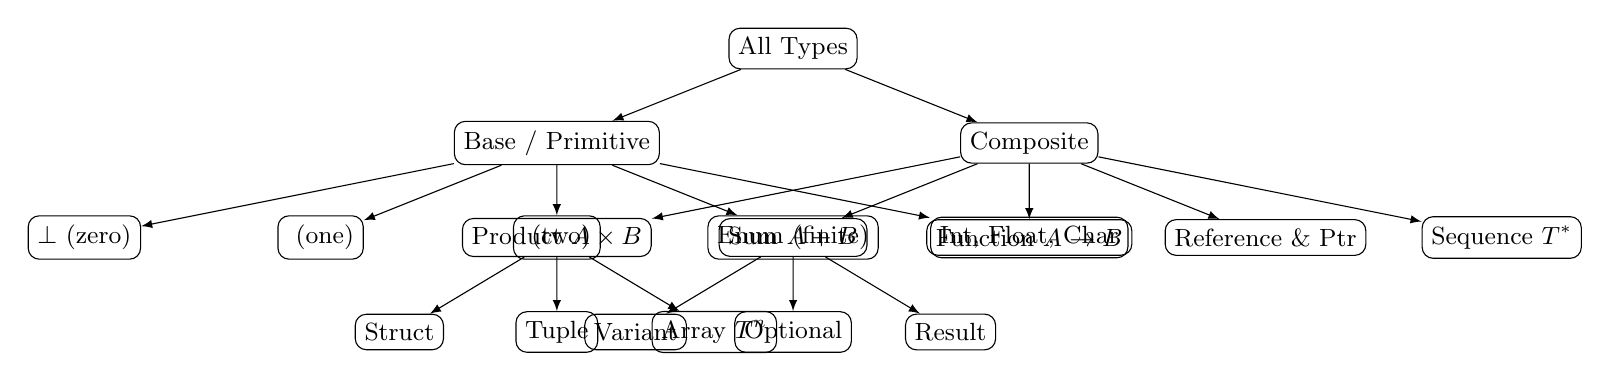
\begin{tikzpicture}[
  every node/.style={draw, rounded corners, text centered, font=\small},
  level distance=12mm,
  level 1/.style={sibling distance=60mm},
  level 2/.style={sibling distance=30mm},
  level 3/.style={sibling distance=20mm},
  edge from parent/.style={draw, -latex}
]
\node {All Types}
  child { node {Base / Primitive}
    child { node {\(\bot\) (zero)} }
    child { node {\(\Unit\) (one)} }
    child { node {\(\Bool\) (two)} }
    child { node {Enum (finite)} }
    child { node {Int, Float, Char} }
  }
  child { node {Composite}
    child { node {Product \(A \times B\)}
      child { node {Struct} }
      child { node {Tuple} }
      child { node {Array \(T^n\)} }
    }
    child { node {Sum \(A + B\)}
      child { node {Variant} }
      child { node {Optional} }
      child { node {Result} }
    }
    child { node {Function \(A \to B\)} }
    child { node {Reference \& Ptr} }
    child { node {Sequence \(T^*\)} }
  }
;
\end{tikzpicture}
\end{center}

\noindent (If you are reading a version without TikZ rendering, refer to the
description below.)

At the top level, types split into \emph{base types} and \emph{composite types}.
Base types are atomic; composite types are built from other types using
combinators: \(\times\) (AND), \(+\) (OR), \(\to\) (function), or repetition.

\subsection{The Algebraic Summary}

Here is a compact summary of the cardinality formulas for every type we have met:

\begin{center}
\begin{tabular}{lll}
\hline
\textbf{Type} & \textbf{Constructor} & \textbf{Cardinality} \\
\hline
\(\bot\)           & Bottom         & \(0\)              \\
\(\Unit\)          & Unit           & \(1\)              \\
\(\Bool\)          & Boolean        & \(2\)              \\
\(\text{Enum}\{e_1,\ldots,e_n\}\) & Enumeration & \(n\) \\
\(\mathtt{int\_k\_t}\) & Fixed integer  & \(2^k\)         \\
\(A \times B\)     & Product        & \(|A| \cdot |B|\)  \\
\(A + B\)          & Sum            & \(|A| + |B|\)      \\
\(A \to B\)        & Function       & \(|B|^{|A|}\)      \\
\(\mathtt{Optional}(A)\) & Optional & \(|A| + 1\)        \\
\(T^n\)            & Fixed array    & \(|T|^n\)          \\
\(T^*\)            & Sequence       & \(\sum_{n \geq 0} |T|^n\) \\
\hline
\end{tabular}
\end{center}

\begin{keyinsight}[Types are algebra]
The table above reveals that types behave exactly like algebraic expressions,
with cardinality playing the role of numerical value. Product is multiplication,
sum is addition, function is exponentiation, \(\bot\) is zero, and \(\Unit\) is
one. This is not a metaphor --- it is a theorem. The correspondence between
types and arithmetic is exact and exploitable.

For example, note that \(A \times \Unit \cong A\) (multiplying by 1 does
nothing), \(A + \bot \cong A\) (adding 0 does nothing), and
\(A \to \Unit \cong \Unit\) (there is only one function from anything to
the one-element type). These identities are both algebraically obvious and
type-theoretically meaningful.
\end{keyinsight}

\subsection{Isomorphism and Type Equivalence}

Two types \(A\) and \(B\) are \textbf{isomorphic} (written \(A \cong B\)) if
there exist functions \(f : A \to B\) and \(g : B \to A\) such that \(f\) and
\(g\) are inverses of each other. Isomorphic types have the same cardinality, but
the converse is not always true (having the same cardinality is necessary but not
sufficient for isomorphism, depending on what structure you require to be
preserved).

\begin{example}
\(\Bool \times \Bool \cong \{0, 1, 2, 3\}\) (i.e., \code{uint2\_t} if such a
type existed). Both have cardinality 4 and both can be bijected with \{0, 1, 2, 3\}.

\(\Bool \to \Bool \cong \Bool \times \Bool\). There are 4 functions from
\(\Bool\) to \(\Bool\), and also 4 values of \(\Bool \times \Bool\). They are
isomorphic!
\end{example}

Isomorphisms tell you when two different ways of representing data are
interchangeable. This is useful for refactoring: if your current data type is
isomorphic to a simpler one, you might be able to simplify your code.

% ============================================================
\section{Designing with Types --- A Few Principles}
\label{sec:designing-with-types}
% ============================================================

Having catalogued the zoo, let us briefly discuss how to use these animals
wisely.

\subsection{Make Illegal States Unrepresentable}

The most powerful use of the type system is to arrange things so that invalid
program states simply \emph{cannot be expressed}. If a state is not a valid
member of your type, the compiler will reject code that tries to create it.

\begin{lstlisting}[style=cpp]
// Bad: both fields can be set, but only one should be active
struct Connection {
    bool is_tcp;
    int  tcp_port;      // valid only if is_tcp
    std::string pipe_name;  // valid only if !is_tcp
};

// Good: the type enforces the mutual exclusion
struct TcpConnection  { int port; };
struct PipeConnection { std::string name; };
using Connection = std::variant<TcpConnection, PipeConnection>;
\end{lstlisting}

In the second version, a \code{Connection} value is \emph{always} either a TCP
connection or a pipe connection --- never some confused mixture. The type makes
the invariant automatic.

\subsection{Prefer Specific Types Over General Ones}

\begin{lstlisting}[style=cpp]
// Vague: what does int mean here? Positive? Bounded?
void set_timeout(int ms);

// Better: the type communicates intent
using Milliseconds = uint32_t;
void set_timeout(Milliseconds ms);

// Even better in C++11+: strong typedef
struct Milliseconds {
    explicit Milliseconds(uint32_t v) : value(v) {}
    uint32_t value;
};
void set_timeout(Milliseconds ms);
// set_timeout(500);               // Compile error!
set_timeout(Milliseconds{500});    // Correct and clear
\end{lstlisting}

\subsection{The Sum-of-Products Pattern}

Many real-world data structures are best expressed as a sum of products: an
outer \code{variant} (sum type) whose alternatives are \code{struct}s (product
types). This is the standard approach in Haskell and is increasingly idiomatic
in modern C++.

\begin{lstlisting}[style=cpp]
struct Circle    { double radius; };
struct Rectangle { double width, height; };
struct Triangle  { double base, height; };

using Shape = std::variant<Circle, Rectangle, Triangle>;

double area(const Shape& s) {
    return std::visit([](const auto& shape) -> double {
        using T = std::decay_t<decltype(shape)>;
        if constexpr (std::is_same_v<T, Circle>)
            return 3.14159 * shape.radius * shape.radius;
        else if constexpr (std::is_same_v<T, Rectangle>)
            return shape.width * shape.height;
        else
            return 0.5 * shape.base * shape.height;
    }, s);
}
\end{lstlisting}

% ============================================================
\section{Summary}
\label{sec:type-zoo-summary}
% ============================================================

We have covered a lot of ground. Here is a rapid recap:

\begin{itemize}
  \item \textbf{Primitive types} (\code{int}, \code{float}, \code{char},
        \code{bool}) are the atoms. Their cardinalities are powers of two.
  \item \textbf{The unit type} \(\Unit\) has exactly one value and carries no
        information. \code{void} in C++ plays this role, imperfectly.
  \item \textbf{The bottom type} \(\bot\) has zero values. It types computations
        that never return. \code{[[noreturn]]} in C++.
  \item \textbf{Booleans} have two values and correspond directly to classical
        logic. Cardinality 2.
  \item \textbf{Enumerations} are finite named sets. Cardinality equals the
        number of enumerators. Use \code{enum class}.
  \item \textbf{Product types} (\code{struct}, \code{tuple}, \code{pair},
        \code{array}) combine types with AND. Cardinality multiplies.
  \item \textbf{Sum types} (\code{variant}, \code{optional}, \code{expected})
        combine types with OR. Cardinality adds. Always prefer tagged over
        untagged unions.
  \item \textbf{Function types} \(A \to B\) classify functions. Cardinality is
        \(|B|^{|A|}\).
  \item \textbf{Pointer and reference types} refer to other values. Smart
        pointers encode ownership in the type.
  \item \textbf{Array and sequence types} collect multiple values of the same
        type. Fixed arrays (\code{std::array}) have size in the type;
        dynamic sequences (\code{std::vector}) have runtime size.
\end{itemize}

\begin{takeaway}[The algebraic nature of types]
Types obey algebraic laws. The combinators \(\times\), \(+\), \(\to\) behave
like multiplication, addition, and exponentiation on cardinalities. \(\bot\) is
zero, \(\Unit\) is one, and \(\Bool\) is two. Understanding these laws lets you
reason about data representations, count states, detect redundancy, and design
types that make illegal states literally unrepresentable. This algebraic view ---
types as numbers, type constructors as operations --- is one of the most
productive ideas in all of type theory.
\end{takeaway}

% ============================================================
\section{Exercises}
\label{sec:type-zoo-exercises}
% ============================================================

\begin{exercise}
\textbf{Cardinality practice.} Compute the cardinality of each of the following
types, showing your work:
\begin{enumerate}[label=(\alph*)]
  \item \code{std::pair<uint8\_t, bool>}
  \item \code{std::variant<bool, uint8\_t>}
  \item \code{std::optional<bool>}
  \item \code{std::array<bool, 10>}
  \item \code{std::function<bool(bool, bool)>} (i.e., the type
        \(\Bool \times \Bool \to \Bool\))
\end{enumerate}
\end{exercise}

\begin{exercise}
\textbf{Making illegal states unrepresentable.} Consider a network packet header
that has a \code{type} field (either \code{DATA} or \code{ACK}) and a
\code{payload\_size} field that is relevant only for \code{DATA} packets
(for \code{ACK} packets, there is no payload). Currently modeled as:
\begin{lstlisting}[style=cpp]
struct Packet {
    enum class Type { DATA, ACK } type;
    uint32_t payload_size;  // only meaningful if type == DATA
};
\end{lstlisting}
Redesign this using a sum-of-products approach with \code{std::variant} so that
\code{payload\_size} cannot be accessed for \code{ACK} packets. What is the
cardinality of the original type? Of your redesigned type?
\end{exercise}

\begin{exercise}
\textbf{Boolean function enumeration.} List all 16 distinct functions of type
\(\Bool \times \Bool \to \Bool\). For each, determine which has a common name
(AND, OR, XOR, etc.). Can you identify functions with no common name?
\end{exercise}

\begin{exercise}
\textbf{Algebraic identities.} Prove each of the following type isomorphisms by
constructing explicit conversion functions in C++ (i.e., write \code{to} and
\code{from} functions that are inverses):
\begin{enumerate}[label=(\alph*)]
  \item \(\Bool \cong \Unit + \Unit\)
        (i.e., \code{bool} $\cong$ \code{std::variant<std::monostate, std::monostate>})
  \item \code{std::optional<A>} $\cong$ \code{std::variant<A, std::monostate>}
  \item \code{std::pair<A, B>} $\cong$ \code{std::pair<B, A>} (commutativity of product)
\end{enumerate}
\end{exercise}

\begin{exercise}
\textbf{The Unit function.} How many functions of type \(A \to \Unit\) are there,
for any type \(A\)? Prove your answer. What does this tell you about using
\(\Unit\) as a return type?
\end{exercise}

\begin{exercise}
\textbf{Bottom in practice.} Write a C++ function template \code{absurd} with
signature:
\begin{lstlisting}[style=cpp]
template <typename T>
T absurd(/* what goes here? */);
\end{lstlisting}
that models the type-theoretic \(\text{absurd} : \bot \to T\). What type should
the parameter have? What should the body of the function be? Why can the body
be empty (or why must it be something specific)?
\end{exercise}

\begin{exercise}
\textbf{Type design challenge.} You are designing a type to represent the state
of a traffic light. The light can be in one of three phases: red (with a
countdown in seconds until it turns green), yellow (always brief, no countdown
needed), or green (with a countdown in seconds until it turns yellow). Design this
type using appropriate sum and product types. Compute its cardinality. Write a
\code{next\_state} function that advances the light to the next phase.
\end{exercise}

\begin{exercise}
\textbf{Function type cardinality.} Compute and compare:
\begin{enumerate}[label=(\alph*)]
  \item \(|\Unit \to A|\) for any type \(A\).
  \item \(|A \to \Unit|\) for any type \(A\).
  \item \(|\bot \to A|\) for any type \(A\).
  \item \(|A \to \bot|\) for any type \(A\) with \(|A| > 0\).
\end{enumerate}
What is special about the answers to (c) and (d)?
\end{exercise}
